\chapter{Introducción}
\section{La energía.}
La energía se puede estudiar desde múltiples puntos de vista (científica, tecnológica, económica, social, ambiental, ético, salud y seguridad).

\subsection{Definición Termodinámica.}
La energía es la capacidad de un sistema para realizar un trabajo.

\subsubsection{Primer principio de la termodinámica.}
\begin{equation}
    \Delta E = Q - W
\end{equation}
La energía de un sistema se convierte en calor ($Q$) y trabajo ($W$) en un proceso termodinámico.

\subsubsection{Segundo principio de la termodinámica.}
\begin{equation}
    \Delta S = \int_{T_1}^{T_2}{\frac{dQ}{T}}
\end{equation}
Determina el sentido de un proceso termodinámico y clasifica la energía según su calidad.

\subsection{Flujos de energía terrestres.}
La potencia total media recibida de la irradiación solar es de $175.000 TW$. La potencia antropogénica es de $18 TW$ (aprox. $2,5 kW/persona$).

\begin{figure}[h]
    \centering
    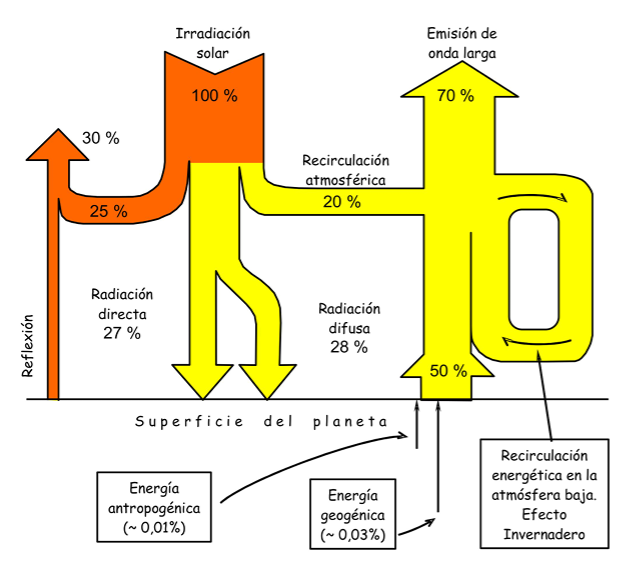
\includegraphics[width=\linewidth]{Imagenes/Flujos de energia terrestres.png}
\end{figure}

\subsection{Exergía.}
La exergía es la parte útil de la energía con la que somos capaces de realizar algún trabajo y obtener servicios basados en la energía. La exergía proviene de sustancias naturales que contienen energía. Mientras que la energía se conserva, la exergía puede destruirse cuando se realiza alguna conversión de energía.

\begin{figure}[h]
    \centering
    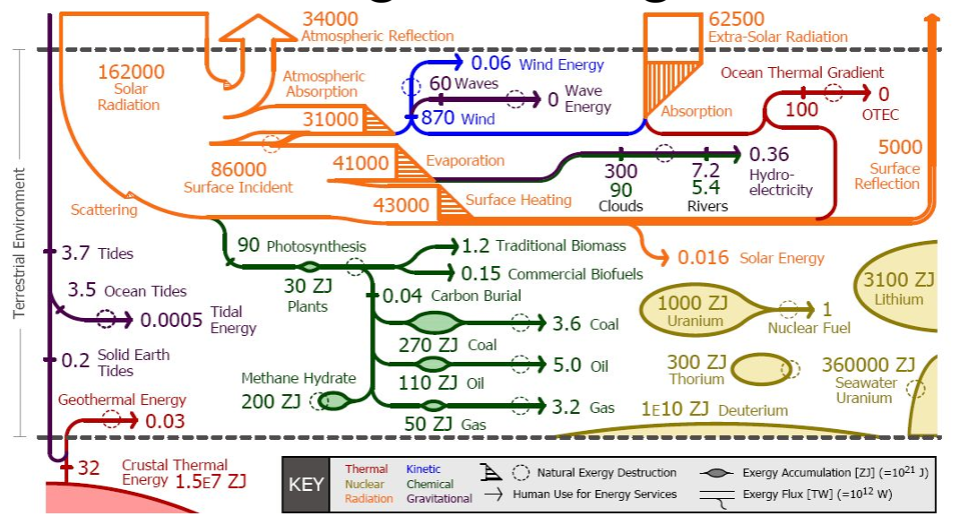
\includegraphics[width=\linewidth]{Imagenes/Exergia.png}
\end{figure}

\subsection{Otros puntos de vista de la energía.}
La energía está ahí cuando el mundo cambia, siempre tiene un papel cuando algo se transforma. La energía no es otra cosa que la unidad de transformar el mundo que nos rodea.

\subsection{Relación con la calidad de vida.}
El ser humano tiene necesidades que desea cubrir. Nuestra sociedad crea o inventa nuevas necesidades continuamente. Parte de estas necesidades se colman con bienes y servicios.

La producción de estos bienes y servicios necesita tomar los medios necesarios de nuestro entorno, transformarlos para hacerlos útiles a nuestras necesidades y acercarlos a las áreas donde serán utilizados. Y para realizar todo esto necesitamos energía.

Por tanto existe una relación entre la calidad de vida y la facilidad del acceso de la energía.
\begin{itemize}
    \item Abundante
    \item Barata
    \item Bien repartida
    \item Moderna
    \item Saludable
\end{itemize}

\subsection{Relación con la economía.}
La energía es un bien escaso (bien económico), y la economía es la ciencia que estudia los bienes económicos, su producción, reparto e intercambio y la generación de riqueza a partir de unos recursos escasos para satisfacer las necesidades humanas local o globalmente.

La energía está ligada a cualquier proceso de transformación y producción de bienes y servicios que cubran las necesidades humanas por lo que es un bien estratégico.

El crecimiento económico de un país está condicionado a su acceso a fuentes de energía.

El precio de la energía tiene un alto contenido ``político'' (déficit de tarifa en el Sector Eléctrico).

\subsection{Relación con el medio ambiente.}
La Tierra es un sistema en equilibrio, por lo que toda la energía que entra por la atmósfera (principalmente radiación solar) es reflejada o transformada y finalmente es emitida espacio exterior como radiación infrarroja.

\begin{itemize}
    \item Balance de energía: El uso de combustibles fósiles produce un desequilibrio en el balance energético.
    \item Balance de masa: Las propiedades ópticas de la atmósfera son las que determinan en última instancia la temperatura de equilibrio. Estas propiedades dependen de la composición de la atmósfera.
\end{itemize}

La obtención de energía de las fuentes naturales siempre produce un impacto sobre el entorno.

\subsection{Ciclo del CO2.}
El balance del CO2 es muy sensible a las actividades humanas. Las propiedades ópticas (reflectividad, transmitancia) de la atmósfera varían de manera muy sensible frente a pequeñas variaciones de su composición (emisiones de Gases Efecto Invernadero).

\subsection{Calentamiento global por $CO_2$ equivalente.}

\subsection{Efectos del calentamiento global.}

\subsection{Objetivos de Desarrollo Sostenible.}
\subsubsection{Energía sostenible y no contaminante.}
¿Por qué ``Energía sostenible y no contaminante'' es un ODS?. El 13\% de la población mundial aún no tiene acceso a servicios modernos de electricidad. 3000 millones de personas dependen de la madera, el carbón, el carbón vegetal o los desechos de origen animal para cocinar y calentar la comida. La energía es el factor que contribuye principalmente al cambio climático y representa alrededor del 60\% de todas las emisiones mundiales de gases de efecto invernadero. La contaminación del aire en locales cerrados debido al uso de combustibles para energía doméstica causó 4,3 millones de muertes en 2012, 6 de cada 10 de estas fueron mujeres y niñas. En 2015, el 17,5\% del consumo final de energía fue de energías renovables.

Los modelos no sostenibles de producción y consumo de energía amenazan la salud y la calidad de vida, al tiempo que afectan los ecosistemas y contribuyen al cambio climático. Por lo tanto, la energía sostenible puede ser un motor en la reducción de la pobreza, progreso social, equidad, resiliencia, crecimiento económico y sostenibilidad medioambiental. Es necesario apoyar y promover una transformación del mercado del sector de la energía a través de una serie de intervenciones políticas, finanzas, creación de capacidades y concientización. Promoviendo las inversiones que ayudan a obtener productos y servicios de energía sostenible, y reduciendo el riesgo del entorno político y financiero, ayudamos a crear el contexto socio-económico por el cual la energía sostenible es posible y viable.

\begin{itemize}
    \item 7.1 De aquí a 2030, garantizar el acceso universal a servicios energéticos asequibles, fiables y modernos.
    \item 7.2 De aquí a 2030, aumentar considerablemente la proporción de energía renovable en el conjunto de fuentes energéticas.
    \item 7.3 De aquí a 2030, duplicar la tasa mundial de mejora de la eficiencia energética.
    \item 7.a De aquí a 2030, aumentar la cooperación internacional para facilitar el acceso a la investigación y la tecnología relativas a la energía limpia, incluidas las fuentes renovables, la eficiencia energética y las tecnologías avanzadas y menos contaminantes de combustibles fósiles, y promover la inversión en infraestructura energética y tecnologías limpias.
    \item 7.b De aquí a 2030, ampliar la infraestructura y mejorar la tecnología para prestar servicios energéticos modernos y sostenibles para todos en los países en desarrollo, en particular los países menos adelantados, los pequeños estados insulares en desarrollo y los países en desarrollo sin litoral, en consonancia con sus respectivos programas de apoyo.
\end{itemize}

\subsubsection{ODS11 y ODS13}

\paragraph{ODS11.}
Las ciudades del mundo ocupan solo el 3\% de la tierra, pero representan entre el 60\% y el 80\% del consumo de energía y el 75\% de las emisiones de carbono.

\paragraph{ODS13.}
Entre 1880 y 2012, la temperatura media mundial aumentó 0,85 grados centígrados. Los océanos se han calentado, la cantidad de nieve y de hielo ha disminuido, y ha subido el nivel del mar. Dada la actual concentración y las continuas emisiones de gases de efecto invernadero, es probable que a finales del siglo el incremento de la temperatura mundial supere los 1,5 grados centígrados en comparación con el período comprendido entre 1850 y 1900 en todos los escenarios menos en uno. Si se adopta una amplia gama de medidas tecnológicas y cambios en el comportamiento, aún es posible limitar el aumento de la temperatura media mundial a 2 grados centígrados por encima de los niveles preindustriales.

\section{El hombre y la energía.}

\section{Fuentes de energía.}
\subsection{Definiciones}
En función de su aprovechamiento distinguimos:
\begin{itemize}
    \item Energía primaria: Magnitud de energía contenida en las funetes.
    \item Energía secundaria: Energía que ha sufrido un proceso de transformación para ser utilizada (insumo).
    \item Energía final: La Energía utilizada finalmente por el usuario (consumo).
\end{itemize}

Procesos del Aprovechamiento energético:
\begin{itemize}
    \item Conversión
    \item Transporte
    \item Almacenamiento
    \item Sistema del que hacemos uso
\end{itemize}

Importancia de la eficiencia energética:
\begin{itemize}
    \item Eficiencia del proceso
    \item Mejora de rendimientos
    \item Disminución de pérdidas
\end{itemize}

\subsubsection{Indicadores}

\begin{itemize}
    \item Intensidad energética: Mide los requerimientos energéticos de la actividad económica.
    \begin{equation}
        IE = \frac{Consumo\ de\ energia(tep)}{PIB(M€)}
    \end{equation}
    \item Intensidad de CO2: Dependencia de combustibles fósiles. También puede interpretarse como medida de la diversidad de fuentes de energéticas de una región.
    \begin{equation}
        ICO_2 = \frac{ton CO_2}{Consumo\ de\ energia(tep)}
    \end{equation}
    \item tonCO2/PIB(M€): combinación de los dos anteriores, mide las emisiones de CO2 con respecto al crecimiento económico.
    \begin{itemize}
        \item PIB per cápita: indicador de la ``salud'' económica de un país.
        \item CO2 per cápita: indicador de la ``salud'' medioambiental del país.
    \end{itemize}
\end{itemize}

\subsubsection{Características de una fuente de energía.}
\begin{itemize}
    \item Renovable / No renovable
    \item Recurso / Reserva
    \item Tipo de energía
    \item Localización
    \item Gestionabilidad
    \item Operación y explotación
    \item Maduración tecnológica.
\end{itemize}

Fuente de energía no renovable: la energía almacenada de cualquier forma que se pueda convertir en calor y que finalmente se pierde hacia el espacio.

Fuente de energía renovable: la energía que utilizada con una tasa determinada, ésta se reemplaza con la misma velocidad.

Recurso: Cantidad de energía cuantificada, con perspectiva de estudio. Todos los recursos no están en el mercado, sin rentabilidad económica.

Reserva: Es la cantidad de recurso evaluado en magnitud y económicamente rentables.

\subsubsection{Consumo de energía en España}

\section{Plan Nacional Integrado de Energía y Clima.}
\subsection{Objetivos.}
El PNIEC es la hoja de ruta que ha de conducir al siguiente escenario en 2030:
\begin{itemize}
    \item 21\% de reducción de emisiones de gases de efecto invernadero (GEI) respecto a 1990.
    \item 42\% de renovables sobre el consumo total de energía final, para toda la UE.
    \item 39,6\% de mejora de la eficiencia energética.
    \item 74\% renovable en la generación eléctrica.
\end{itemize}
En 2050 el objetivo es alcanzar la neutralidad climática con la reducción de al menos un 90\% de nuestras emisiones de GEI y en coherencia con la Estrategia Europea. Además de alcanzar un sistema eléctrico 100\% renovable en 2050.

\subsection{Pilares}
El PNIEC de España identifica los retos y oportunidades a lo largo de las cinco dimensiones de la Unión de la Energía:
\begin{enumerate}
    \item La descarbonización, incluidas las energías renovales;
    \item La eficiencia energética;
    \item La seguridad energética;
    \item El mercado interior de la energía y
    \item La investigación, innovación y competitividad.
\end{enumerate}

\section{Tecnología energética.}
\subsection{Tecnologías, Políticas y Meidas para Mitigar el C.C.}
Medidas Potenciales:
\begin{itemize}
    \item Programas basados en el mercado:
    \begin{itemize}
        \item Impuestos sobre el carbono o la energía
        \item Precios en función de la totalidad de los costos
        \item Reducción de subvenciones
        \item Cuotas negociables sobre las emisiones
    \end{itemize}
    \item Acuerdos voluntarios:
    \begin{itemize}
        \item Uso de la energía y normas sobre las emisiones de carbono
        \item Fomento de programas de uso eficiente de la energía
    \end{itemize}
    \item Medidas reglamentarias:
    \begin{itemize}
        \item Equipo obligatorio, normas sobre construcción
        \item Prohibiciones de productos o prácticas
    \end{itemize}
    \item Investigación - Desarrollo y Demostración de nuevas tecnologías
\end{itemize}

\subsection{Tecnologías para reducir las emisiones de GEI}
\begin{itemize}
    \item Conversión más eficiente de combustibles fósiles
    \item Cambio a combustibles fósiles con bajo contenido en carbono
    \item Descarbonización de gases de escape y combustibles
    \item Captura y almacenamiento de CO2
    \item Cambio a energías no emisoras de GEI:
    \begin{itemize}
        \item Energía nuclear
        \item Fuentes renovables
    \end{itemize}
\end{itemize}

Factores:
\begin{itemize}
    \item Rentabilidad económica
    \item Aceptación social
    \item Aprobación política
\end{itemize}